\scanpage{50}%
\mspage{\handwritten{18}}%
nothing, it follows that one of the $K_i$ is already reduced to the trivial group, hence that $G\handwritten{\to}\underline{\operatorname{Aut}}_{\inserted{\handwritten{V_i}}}\deleted{\unsure{(V_i)}}$ is a monomorphism. It is therefore a closed immersion by virtue of (1.4.2), which proves that (iv)$\handwritten{\Rightarrow}$(v). Since (\deleted{g}v)$\handwritten{\Rightarrow}$(i) trivial-\linebreak ly, this proves 11.11\deleted{\unsure{.}} for $G$ of finite type.

\deleted{Let us now take the general case, where it remains to prove that (iv)$\handwritten{\Rightarrow}$(i). With the notation of the preceding proof, let $G_i$ be the\inserted{
\begin{tikzpicture}[x=1cm,y=1cm,baseline=(n.base)]\node (n) at (0,0) {smallest};\draw (-.55,-.18) .. controls (-1.2,-.13) and (-1.2,.35) .. (0,.3) .. controls (1.1,.3) and (1.2,-.2) .. (.2,-.24) .. controls (-.7,-.24) and (-.8,-.2) .. (-.8,-.55);\end{tikzpicture}} closed subgroup of $\operatorname{Aut}(V_i)$ through wh\handwritten{i}ch\inserted{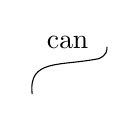
\begin{tikzpicture}[x=1cm,y=1cm,baseline=(n.base)]\node (n) at (0,0) {can};\draw (-.45,-.65) .. controls (-.5,-.2) and (-.1,-.3) .. (.4,-.2) .. controls (.5,-.15) and (.5,-.1) .. (.5,-.05);\end{tikzpicture}} be factored $G\handwritten{\to}\underline{\operatorname{Aut}}_{\inserted{\handwritten{V_i}}}\deleted{(V_i)}$ \deleted{(exists} (such a group exists, \deleted{since} as the intersection of all those through which $G\handwritten{\to}\deleted{\unsure{\operatorname{Aut}(V_i)}}\inserted{\underline{\operatorname{Aut}}_{V_i}}$ factors). If $V_j\handwritten{\supset}V_i$, one then sees at once that $G_j$ preserves $V_i$ , and that the corresponding morphism $G_j\handwritten{\to}\underline{\operatorname{Aut}}_{V_i}$ fac-\linebreak tors through $G_i$ . In this way, the $G_i$ form a projective system of affine grou-\linebreak ps over $k$, and we have a natural morphism $G\handwritten{\longrightarrow}G'=\underset{\handwritten{\longleftarrow}}{\lim}G_i$ , where $G'$ is itself an affine group (EGA IV 8.2.3). The hypothesis that $G$ acts \uline{faithfully} on $V$ is then expressed by\deleted{\unsure{r}} the fact that $G\handwritten{\to}G'$ is a monomor-\linebreak phism. We have thus found\handwritten{\makebox[0pt][l]{\raisebox{-.5ex}{\begin{tikzpicture}[x=.25cm,y=.25cm]\draw (0,-.5)--(.55,1);\end{tikzpicture}}}}a monomorphism from $G$ into an affine scheme, which implies that the quasi-compa\deleted{\unsure{t}}\handwritten{c}t\inserted{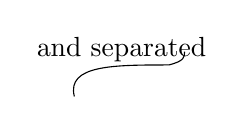
\begin{tikzpicture}[x=1cm,y=1cm,baseline=(n.base)]\node (n) at (0,0) {and separated};\draw (-.6,-.6) .. controls (-.7,-.2) and (-.1,-.2) .. (.6,-.2) .. controls (.8,-.15) and (.8,-.1) .. (.8,-.03);\end{tikzpicture}} scheme $G$ is quasi-affine, i.e. that its structure sheaf is ample, by virtue of EGA IV 18.12.17 . In \handwritten{o}ther terms, setting $H=\operatorname{Spec}\handwritten{\Gamma}(G,\underline{O}_G)$ , the canonical morphism $G\handwritten{\to}H$ is an open immersion. Let us now note that $H$ is naturally a group scheme, and $G\handwritten{\to}H$ a group homomorphism, thanks to 11.2 . This homomorphism is obviously dominant, it remains to prove that it is an isomorphism, which follows\deleted{ra d\unsure{e|a}} from the following lemma:}
\margin{\handwritten{\figure{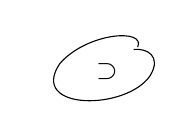
\begin{tikzpicture}
\draw (.39,.31) .. controls (.5,.55) and (-.25,.5) .. (-.6,.1) .. controls (-1,-.5) and (.25,-.5) .. (.55,-.05) .. controls (.7,.2) and (.5,.3) .. (.34,.28);\node at (0,0) {$\supset$};
\end{tikzpicture}}}}

\deleted{\uline{Lemma} 11.11.1.\handwritten{\unsure{,}} Let $\deleted{\unsure{G}}\handwritten{H}$ be a group scheme over a field\inserted{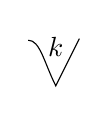
\begin{tikzpicture}[x=1cm,y=1cm,baseline=(n.base)]\node (n) at (0,0) {$k$};\draw (-.35,.08) .. controls (-.2,.08) and (-.15,-.2) .. (0,-.5)--(.3,.1);\end{tikzpicture}}\handwritten{.} \deleted{$G$ a sub-} Then every open subgroup scheme\inserted{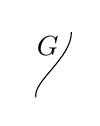
\begin{tikzpicture}[x=1cm,y=1cm,baseline=(n.base)]\node (n) at (0,0) {$G$};\draw (.3,.18) .. controls (.3,-.15) and (-.2,-.45) .. (-.15,-.65);\end{tikzpicture}} of $H$ is also closed.}
\margin{\handwritten{\figure{\begin{tikzpicture}\draw (0,0)--(.03,-.8);\end{tikzpicture}}}}

\deleted{It amounts to the same thing to say that the set $H-G$ is open, i.e. is a neighborhood of each of its points\deleted{,} $x$ . Now , every field extension $k'/k$ defining a morphism $\operatorname{Spec}k'\handwritten{\to}\operatorname{Spec}k$ which is universally}
% archive sheet number: 49
